\begin{document}
  \chapter{Implementation on the Database Management Systems}

    \section{The System}
      \paragraph{}
        In this project, the Database System we're using is MySQL version 5.6.35 hosted locally on our members' laptops as shown in figure. \\
        The project also implemented purely on PHP7.
      \begin{center}
        \begin{figure}
          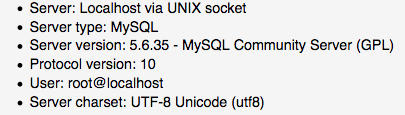
\includegraphics{ch3_1}
          \caption{System Detail}
          \label{sysdetail}
        \end{figure}
      \end{center}
    \section{Workflow and Methodology}
      \paragraph{}
        In order to create continuous flow of the teamworking, team management and planning was very important to us. We used
          ,somewhat, Agile Philosophy in our development cycles. Our group included development team, which included frontend development
          and backend development, and testing team.
      \paragraph{}
        As we split our implementation time into periods and assign tasks to each team, the flow was very smooth and allowed us to work independently most of the time.

      \paragraph{}
        We also used a few tools to help us implement out project more efficiently such as GitHub as Version Control System to keep track of our code and productivity of
        each team members, We also use GitHub readme as Planning Board for our team to plan future work together as we meet together for daily meeting.

      \paragraph{}
        In this project we didnot use any CSS Framework or JS Framework because we believed that learning best should start by learning at the very basic steps.
        So we implement our own CSS library which isn't Well-Refractored but it is the excellent evidence of our learning.

      \paragraph{}
        This reported is written using \LaTeX.

    \section{The Database}
      \paragraph{}
        We planned quite a perfect ER in the very beginning phase of the implementation, but as we continued we need to modify the ER some times because of a few reasons listed below.
        \begin{enumerate}
          \item To support new functional requirements, which are found out while implementing
          \item To facilitate physical implementation
          \item To do some actions that are constrained by the Database System
        \end{enumerate}
      \paragraph{}
        The SQL script of our database is exported and included in the appendix.
        So our final Database includes the following tables.\\
        \newpage
    \begin{center}
      \begin{figure}
        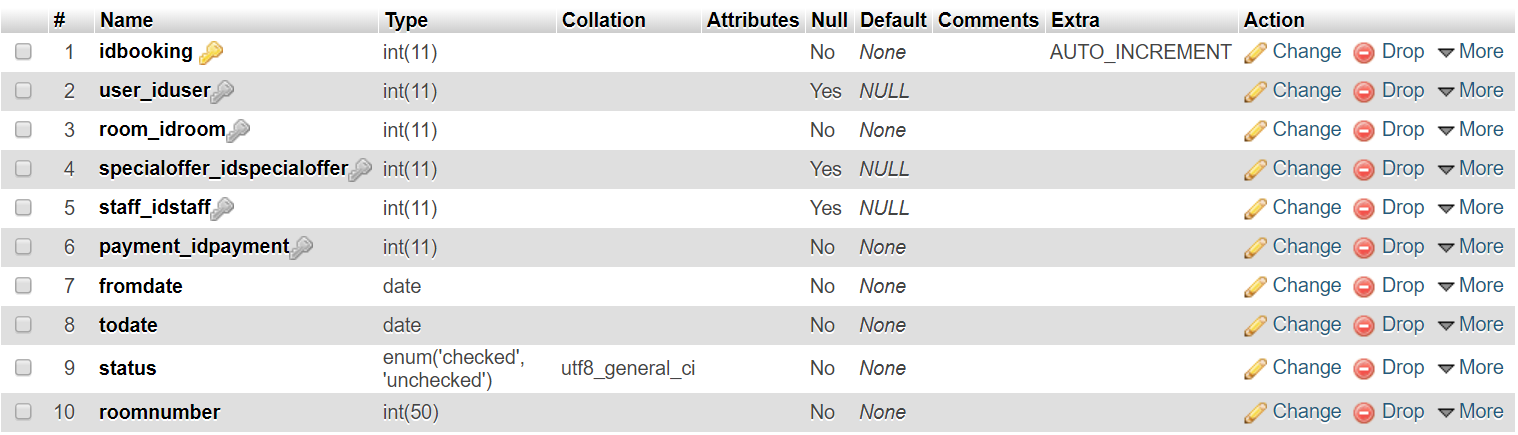
\includegraphics[width=\textwidth]{Booking}
        \caption{Structure of booking table}
      \end{figure}
      \begin{figure}
        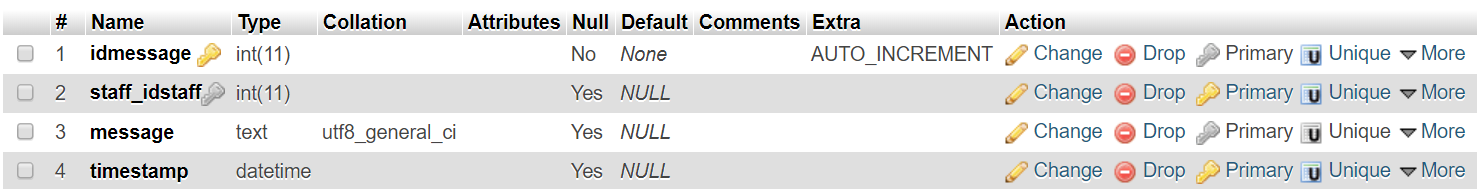
\includegraphics[width=\textwidth]{Message}
        \caption{Structure of message table}
      \end{figure}
      \begin{figure}
        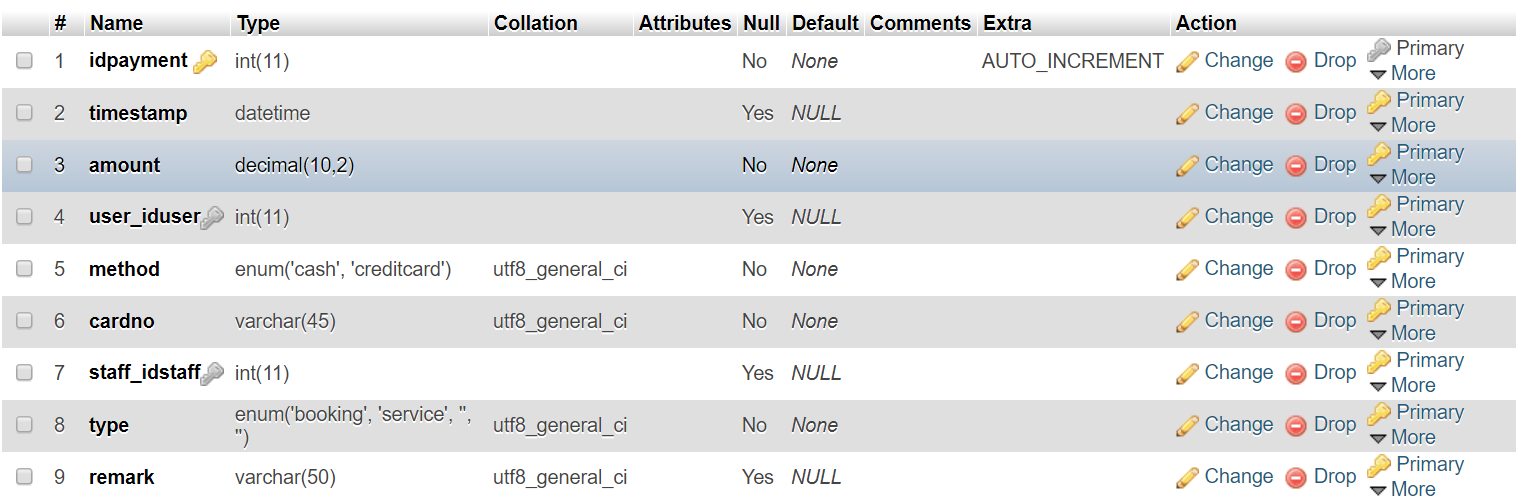
\includegraphics[width=\textwidth]{payment}
        \caption{Structure of payment table}
      \end{figure}
      \begin{figure}
        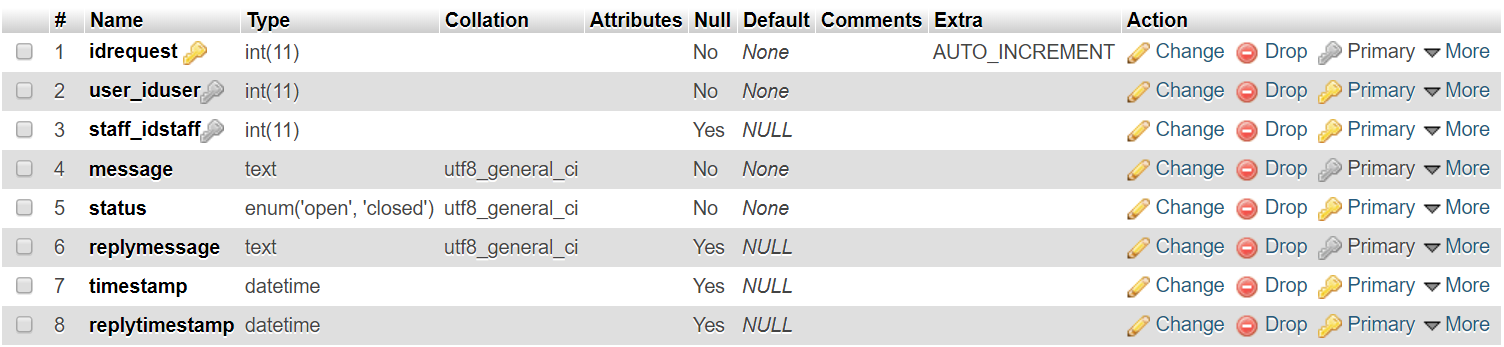
\includegraphics[width=\textwidth]{request}
        \caption{Structure of request table}
      \end{figure}
      \begin{figure}
        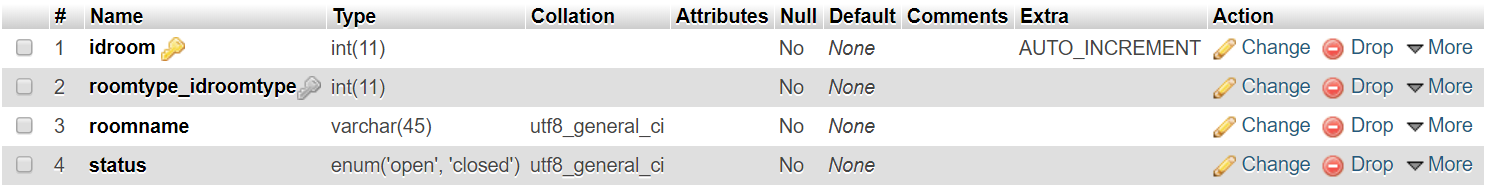
\includegraphics[width=\textwidth]{room}
        \caption{Structure of room table}
      \end{figure}
      \begin{figure}
        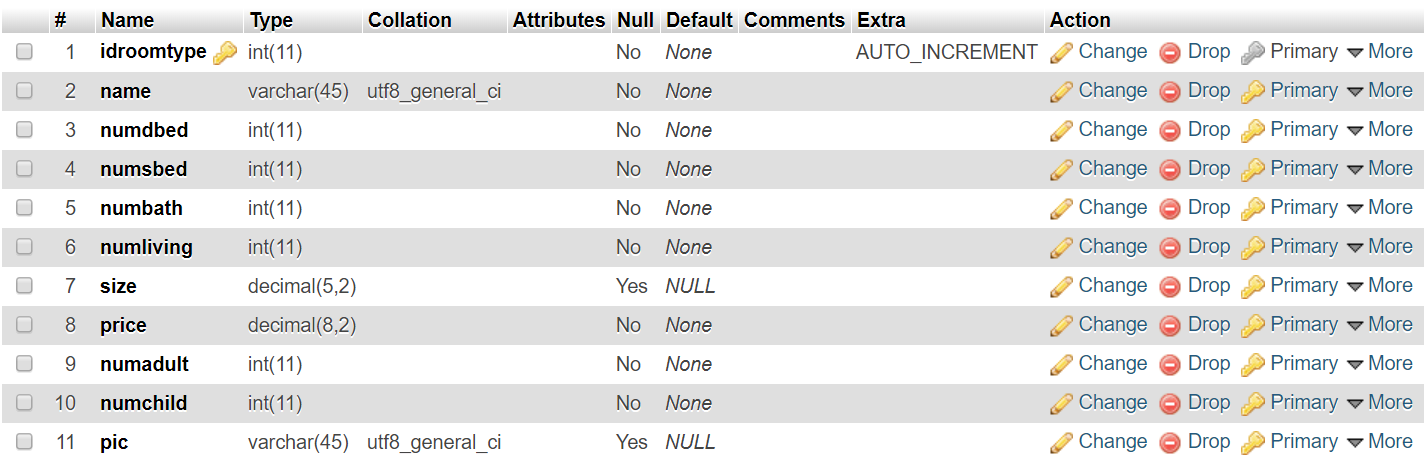
\includegraphics[width=\textwidth]{roomtype}
        \caption{Structure of roomtype table}
      \end{figure}
      \begin{figure}
        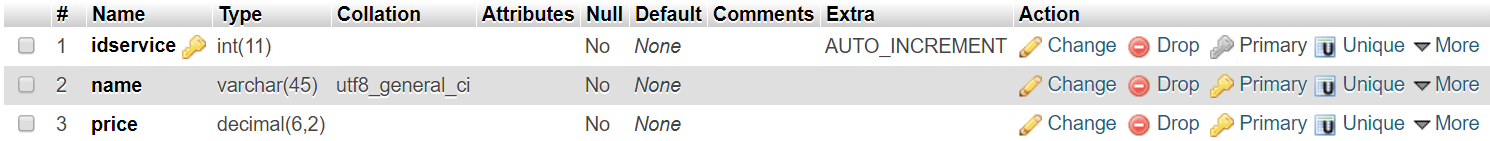
\includegraphics[width=\textwidth]{service}
        \caption{Structure of message table}
      \end{figure}
      \begin{figure}
        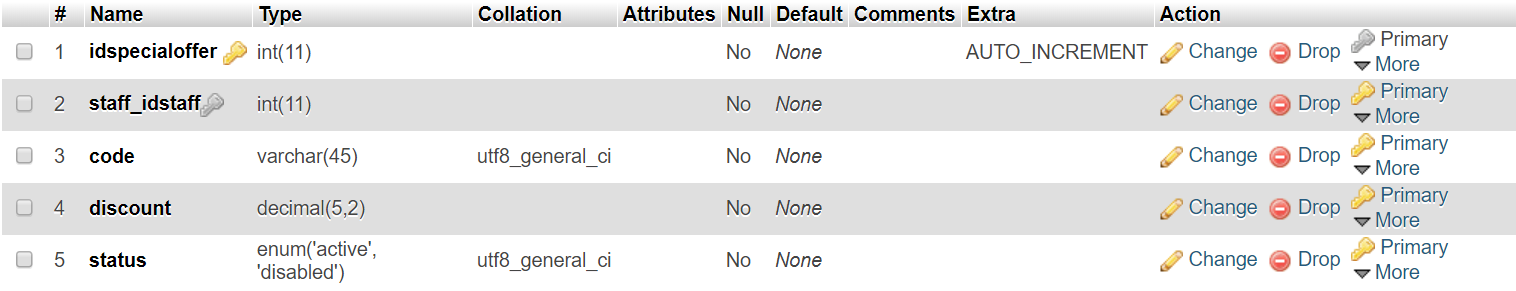
\includegraphics[width=\textwidth]{specialoffer}
        \caption{Structure of specialoffer table}
      \end{figure}
      \begin{figure}
        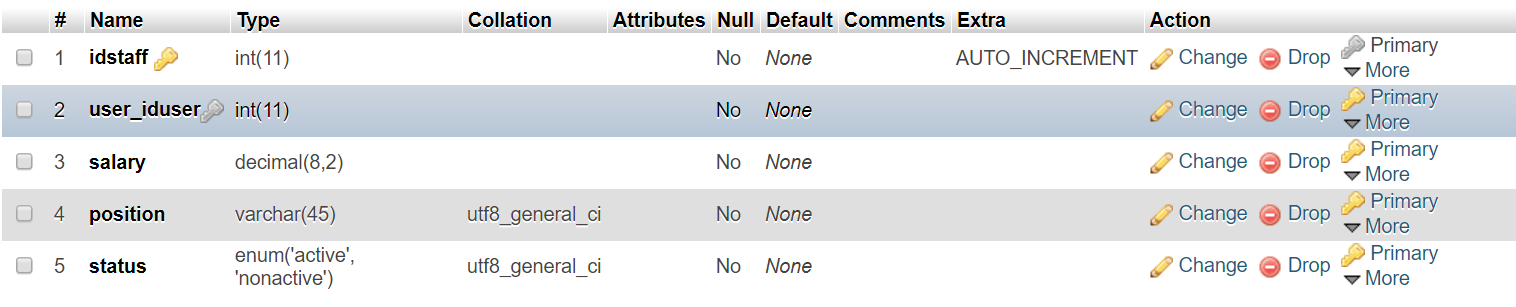
\includegraphics[width=\textwidth]{staff}
        \caption{Structure of staff table}
      \end{figure}
      \begin{figure}
        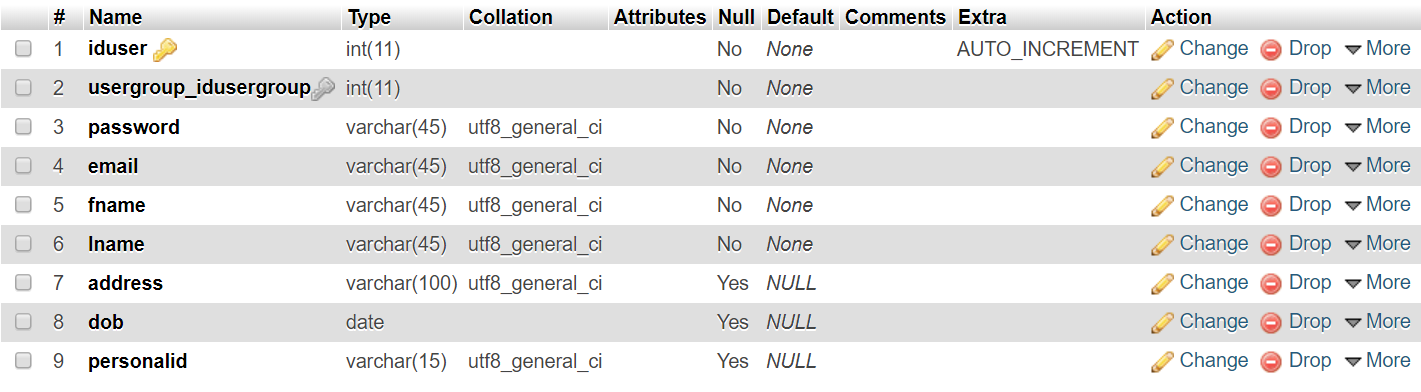
\includegraphics[width=\textwidth]{user}
        \caption{Structure of user table}
      \end{figure}
      \begin{figure}
        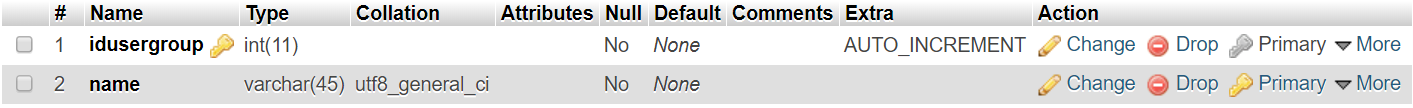
\includegraphics[width=\textwidth]{usergroup}
        \caption{Structure of usergroup table}
      \end{figure}
      \begin{figure}
        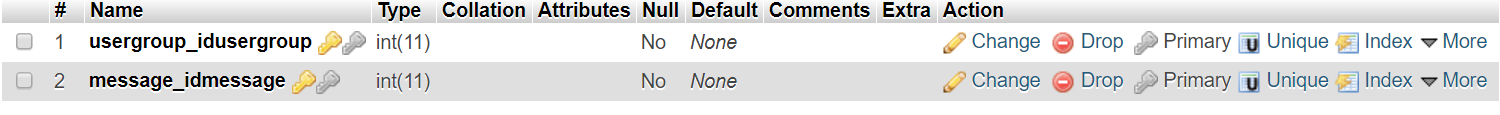
\includegraphics[width=\textwidth]{usergrouphasmessage}
        \caption{Structure of usergroup\_has\_message table}
      \end{figure}
    \end{center}
      \paragraph{}
        We also used a lot of routines, namely stored procedure, functions and trigger, and will be discussed later in the next chapter.\\
\newpage
    \section{The project:The Test Dataset}
      \paragraph{}
        the following tables are the test dataset and currently in our database.\\
        \begin{center}
          \begin{figure}
            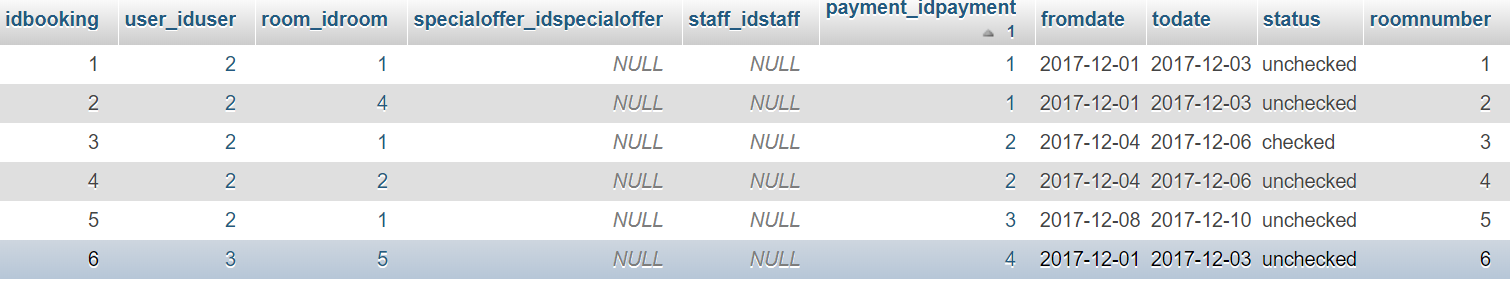
\includegraphics[width=\textwidth]{tsBooking}
            \caption{Test dataset of Booking}
          \end{figure}
          \begin{figure}
            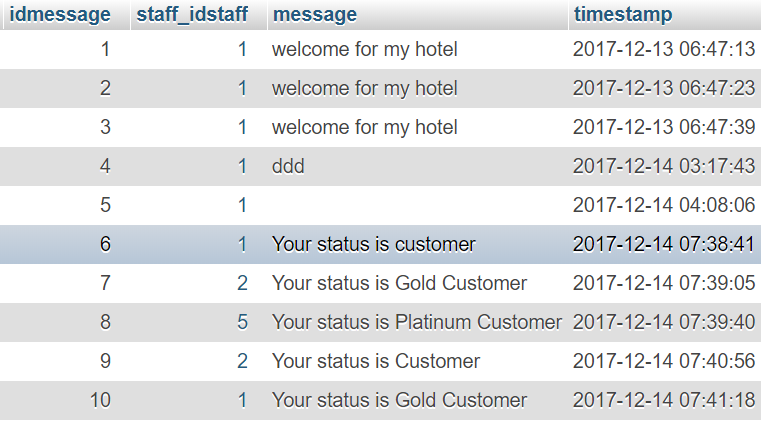
\includegraphics[width=\textwidth]{tsMessage}
            \caption{Test dataset of Message}
          \end{figure}
          \begin{figure}
            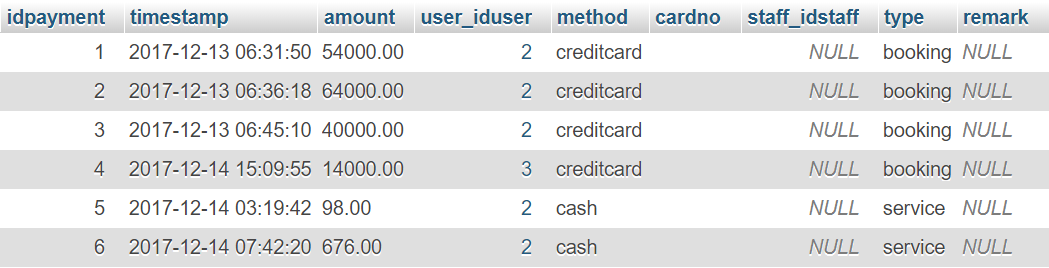
\includegraphics[width=\textwidth]{tsPayment}
            \caption{Test dataset of Payment}
          \end{figure}
          \begin{figure}
            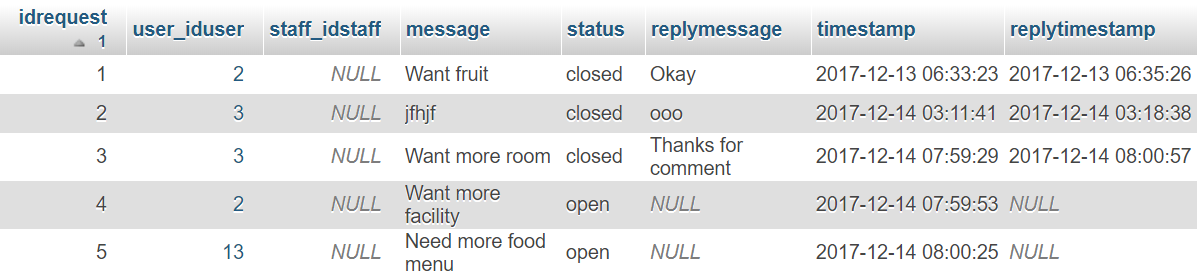
\includegraphics[width=\textwidth]{tsrequest}
            \caption{Test dataset of Request}
          \end{figure}
          \begin{figure}
            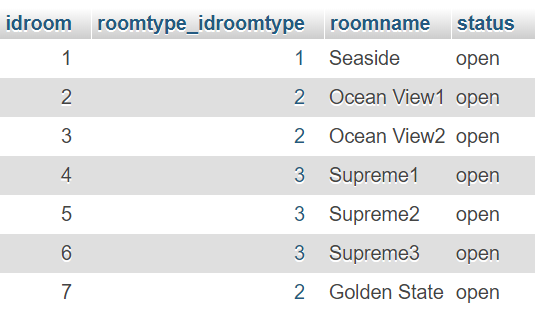
\includegraphics[width=\textwidth]{tsRoom}
            \caption{Test dataset of Room}
          \end{figure}
          \begin{figure}
            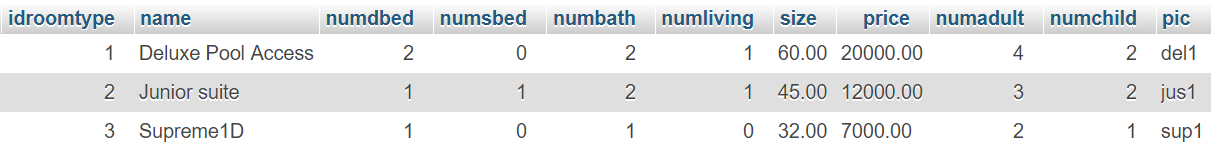
\includegraphics[width=\textwidth]{tsRoomtype}
            \caption{Test dataset of Roomtype}
          \end{figure}
          \begin{figure}
            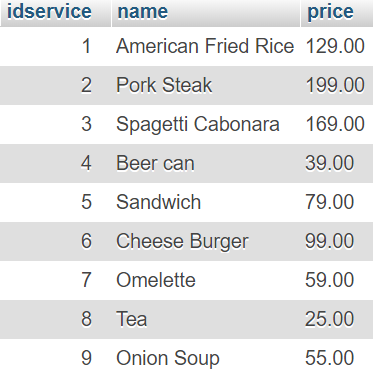
\includegraphics[width=\textwidth]{tsService}
            \caption{Test dataset of Service}
          \end{figure}
          \begin{figure}
            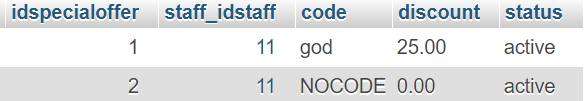
\includegraphics[width=\textwidth]{tsSpecialoffer}
            \caption{Test dataset of SpecialOffer}
          \end{figure}
          \begin{figure}
            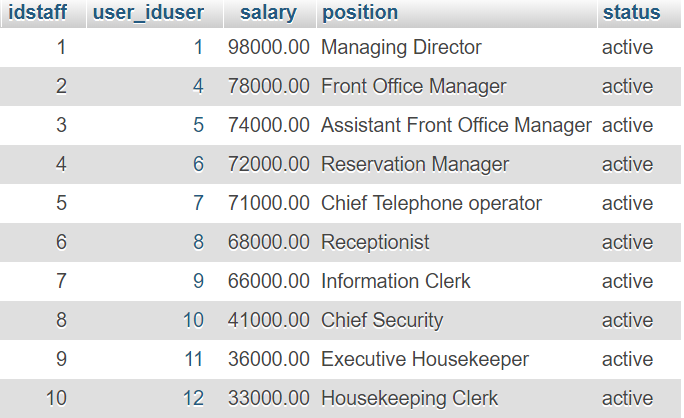
\includegraphics[width=\textwidth]{tsStaff}
            \caption{Test dataset of Staff}
          \end{figure}
          \begin{figure}
            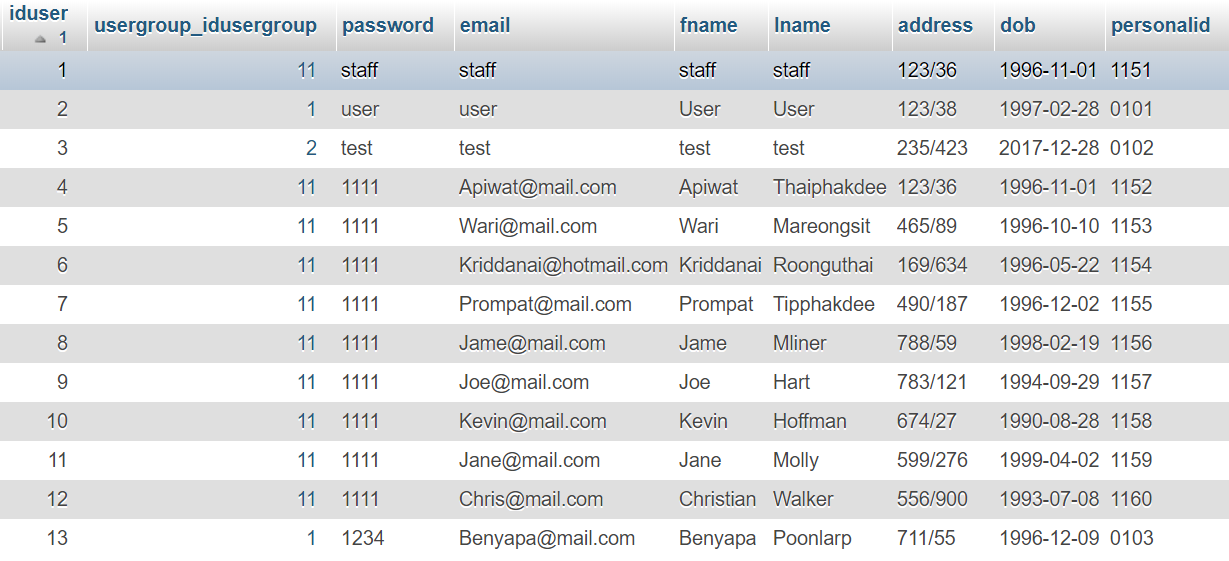
\includegraphics[width=\textwidth]{tsUser}
            \caption{Test dataset of User}
          \end{figure}
          \begin{figure}
            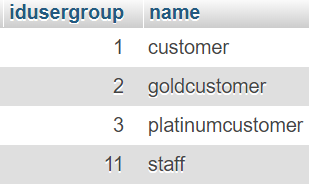
\includegraphics[width=\textwidth]{tsUsergroup}
            \caption{Test dataset of Usergroup}
          \end{figure}
          \begin{figure}
            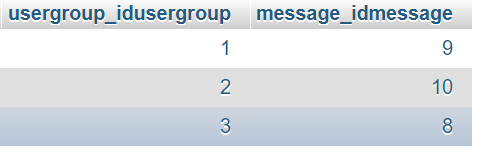
\includegraphics[width=\textwidth]{tsusergrouphasmessage}
            \caption{Test dataset of Usergroup\_has\_message}
          \end{figure}

        \end{center}
        \newpage

        \section{The project : User Interface}

    \begin{center}
      \begin{figure}
        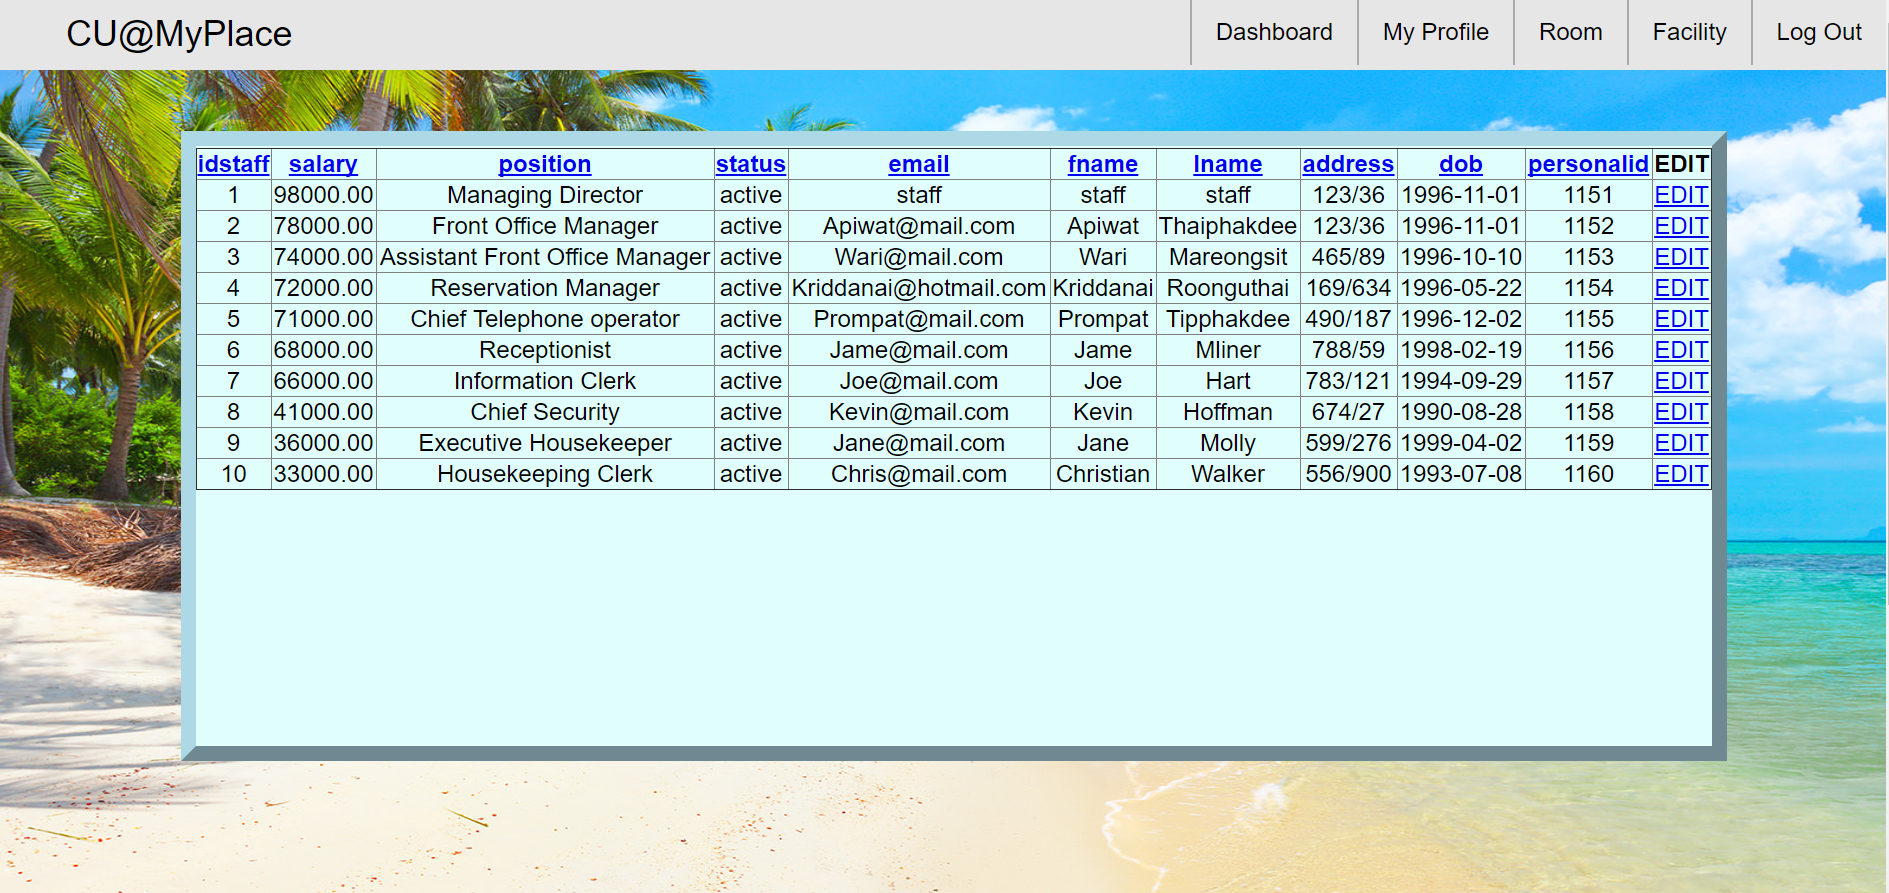
\includegraphics[width=\textwidth]{editstaff}
        \caption{User Interface of Staff Editting}
      \end{figure}
      \begin{figure}
        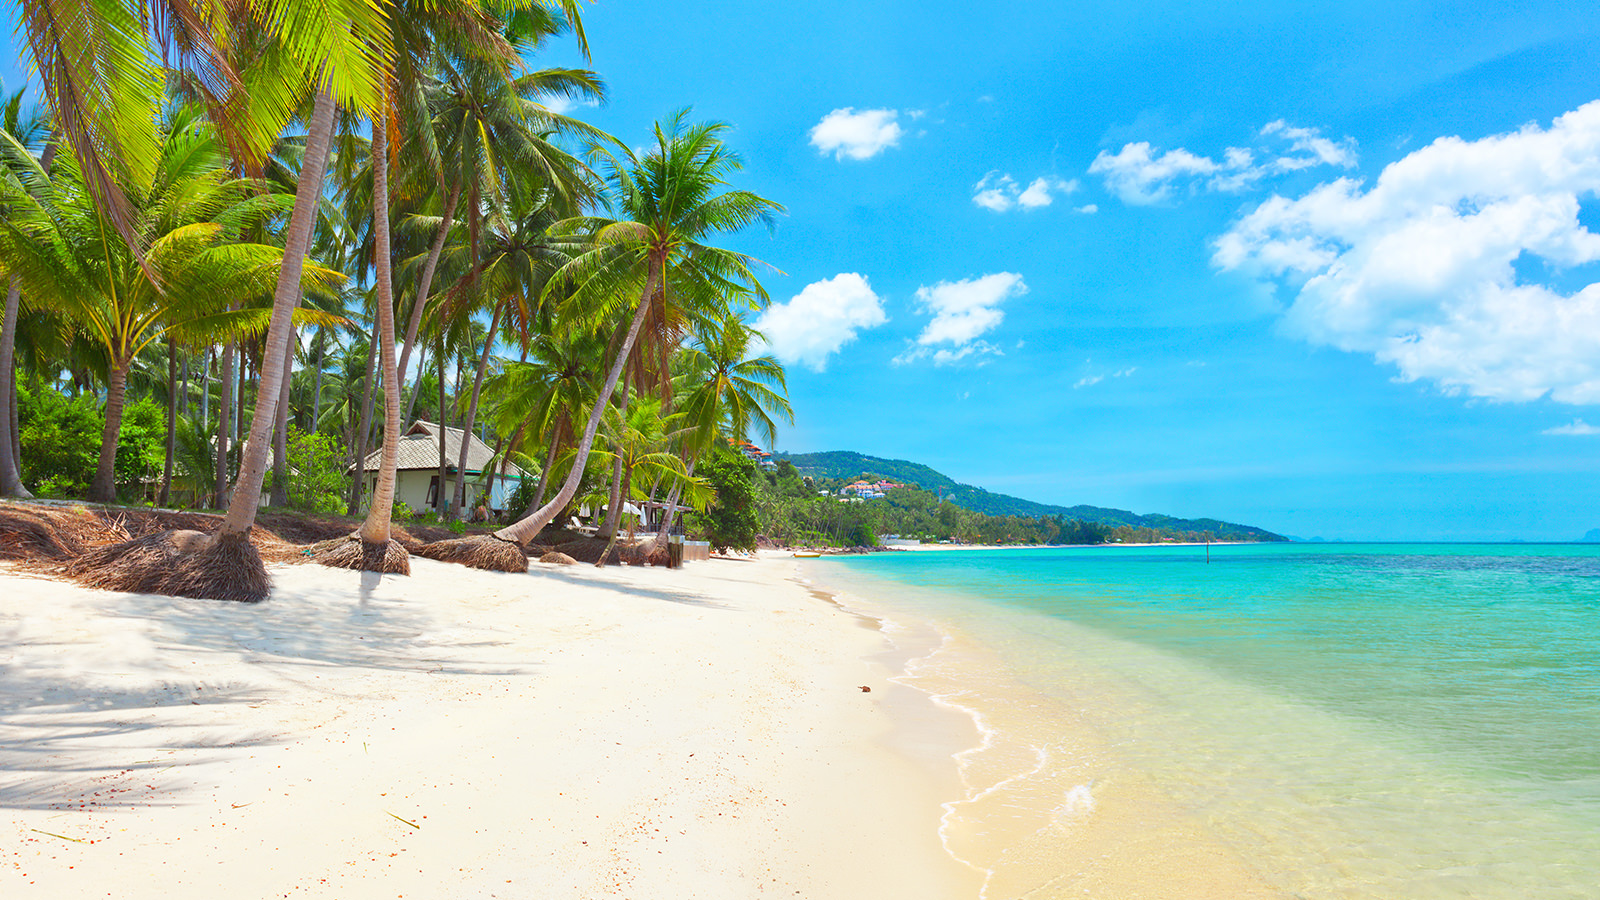
\includegraphics[width=\textwidth]{home1}
        \caption{User Interface of Homepage1}
      \end{figure}
      \begin{figure}
        
\includegraphics[width=\textwidth]{home2}
        \caption{User Interface of Homepage2}
      \end{figure}
      \begin{figure}
        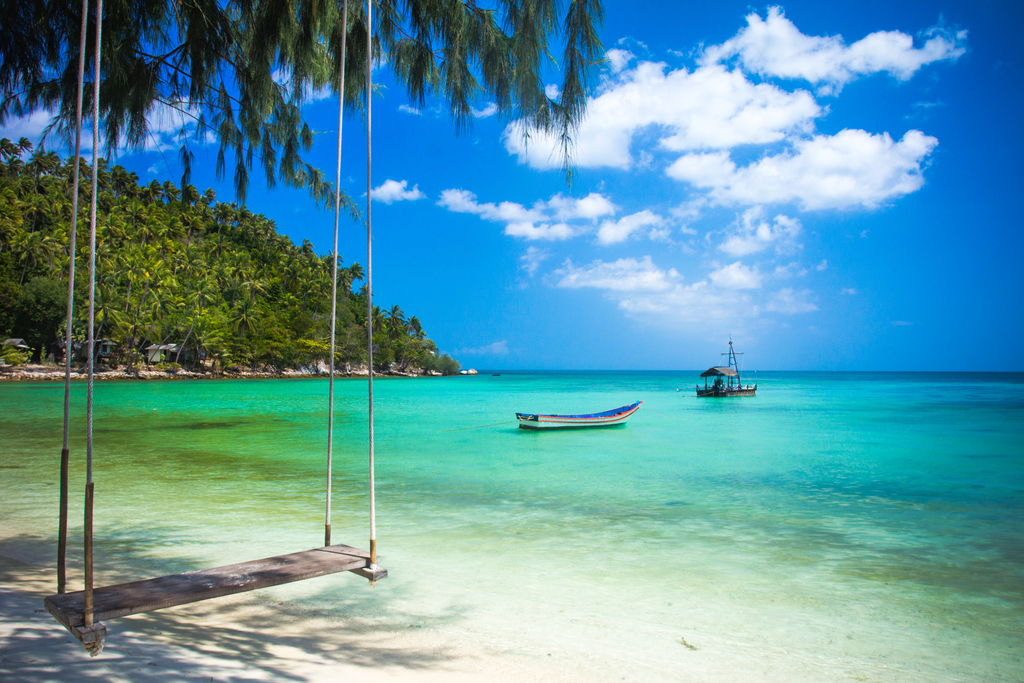
\includegraphics[width=\textwidth]{home3}
        \caption{User Interface of Homepage3}
      \end{figure}
      \begin{figure}
        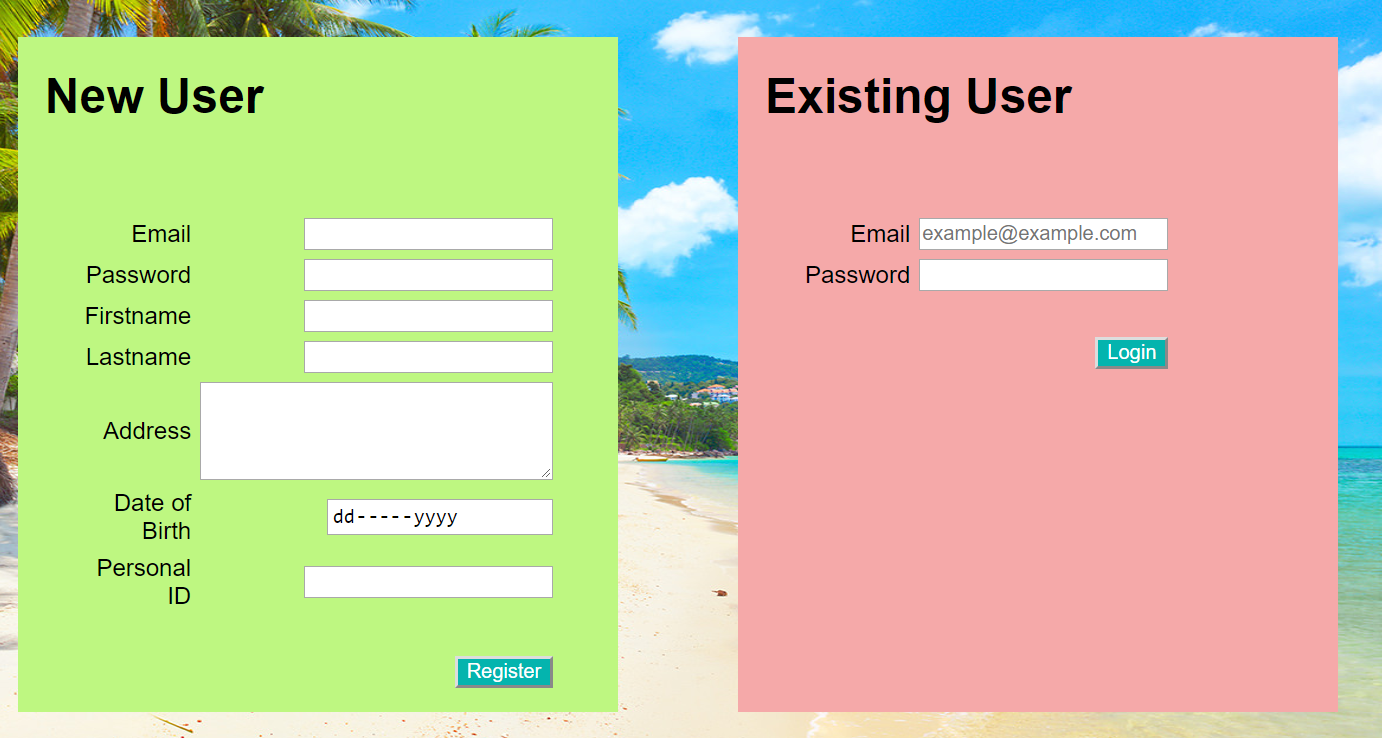
\includegraphics[width=\textwidth]{login}
        \caption{User Interface of login}
      \end{figure}
      \begin{figure}
        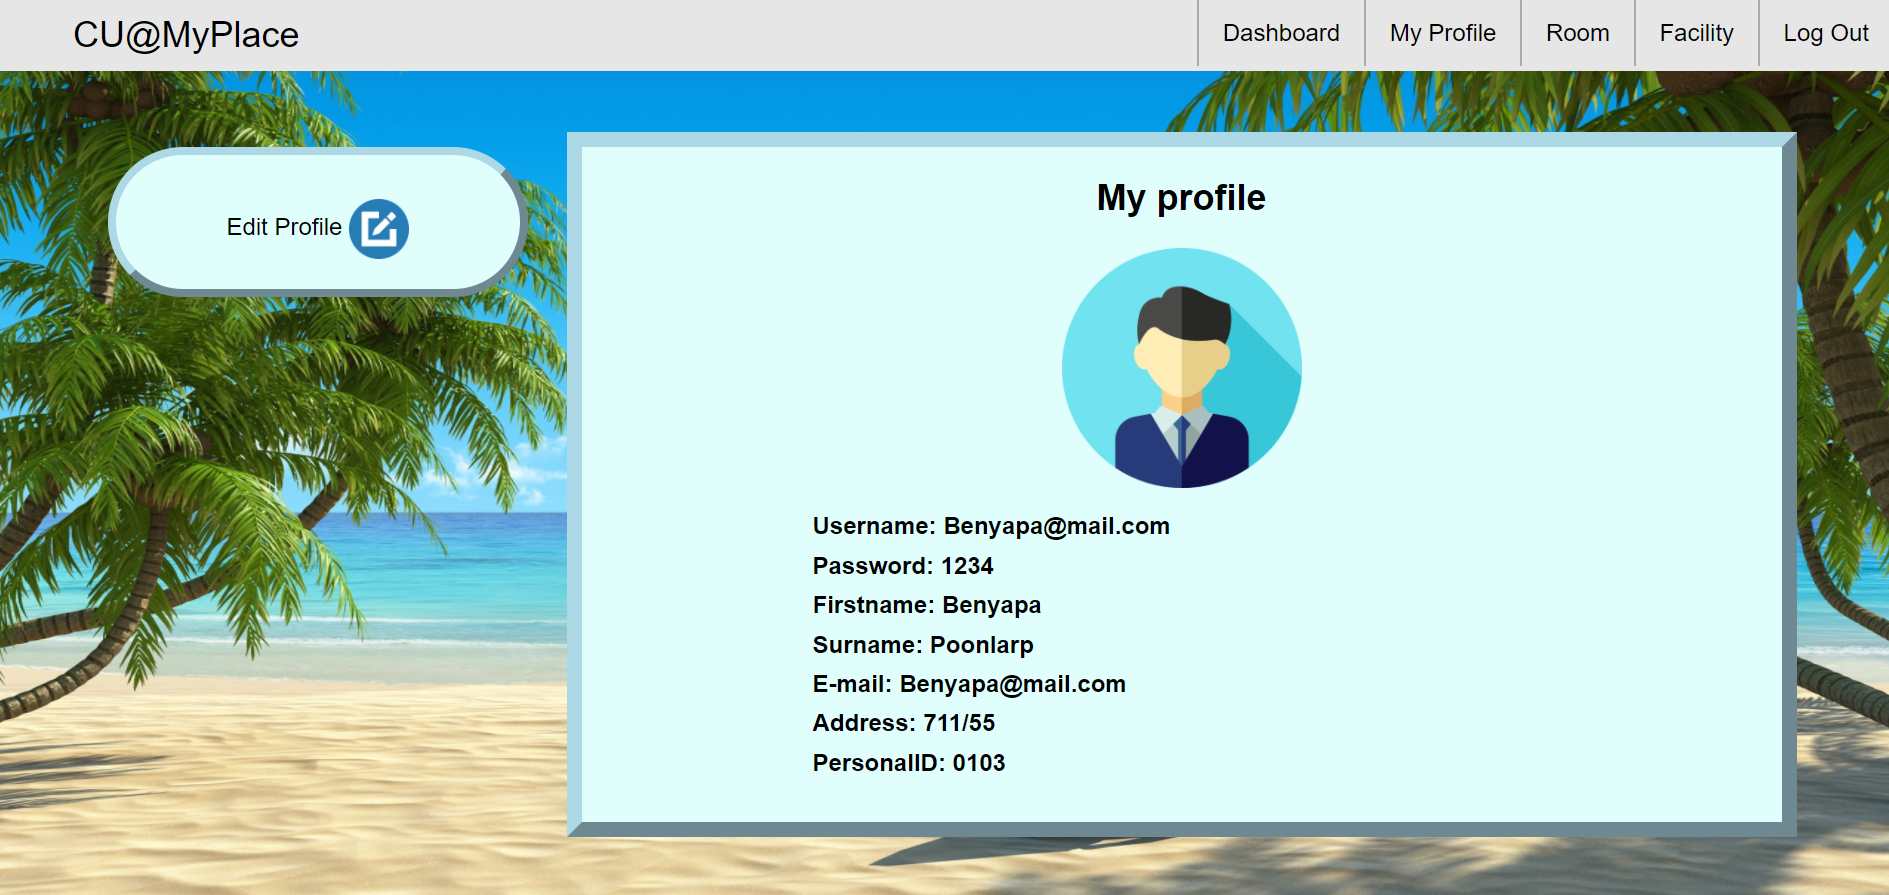
\includegraphics[width=\textwidth]{myprofile}
        \caption{User Interface of myprofile}
      \end{figure}
      \begin{figure}
        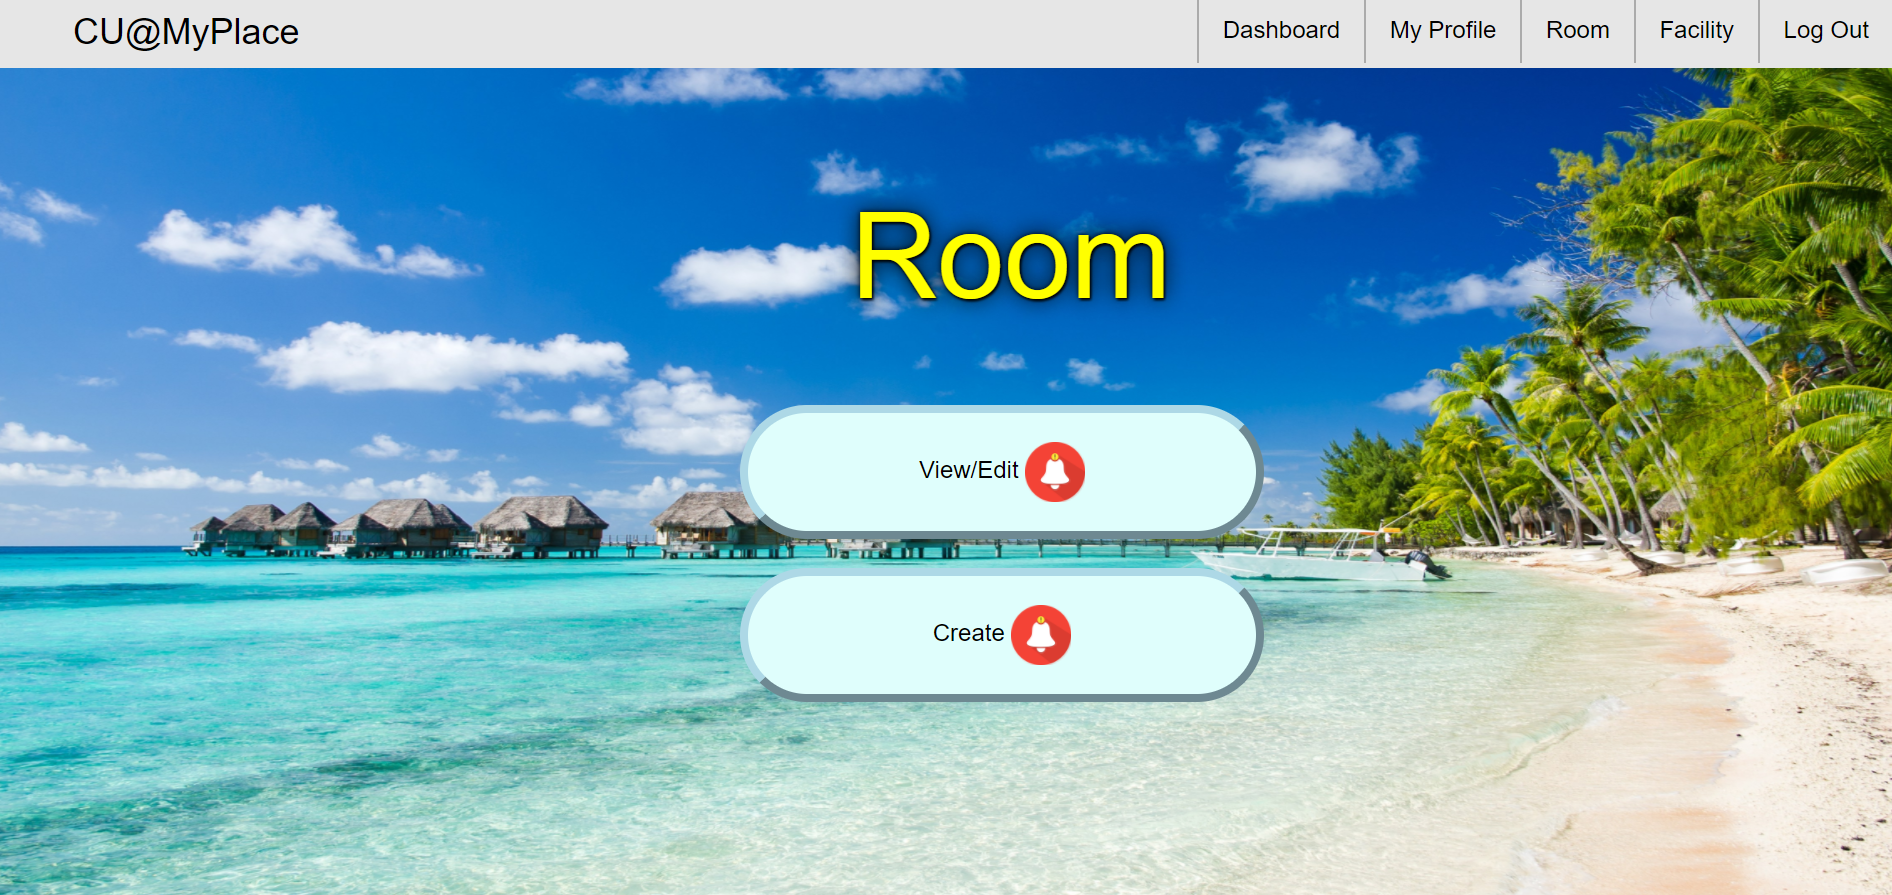
\includegraphics[width=\textwidth]{roomfunction}
        \caption{User Interface of roomfunction}
      \end{figure}
      \begin{figure}
        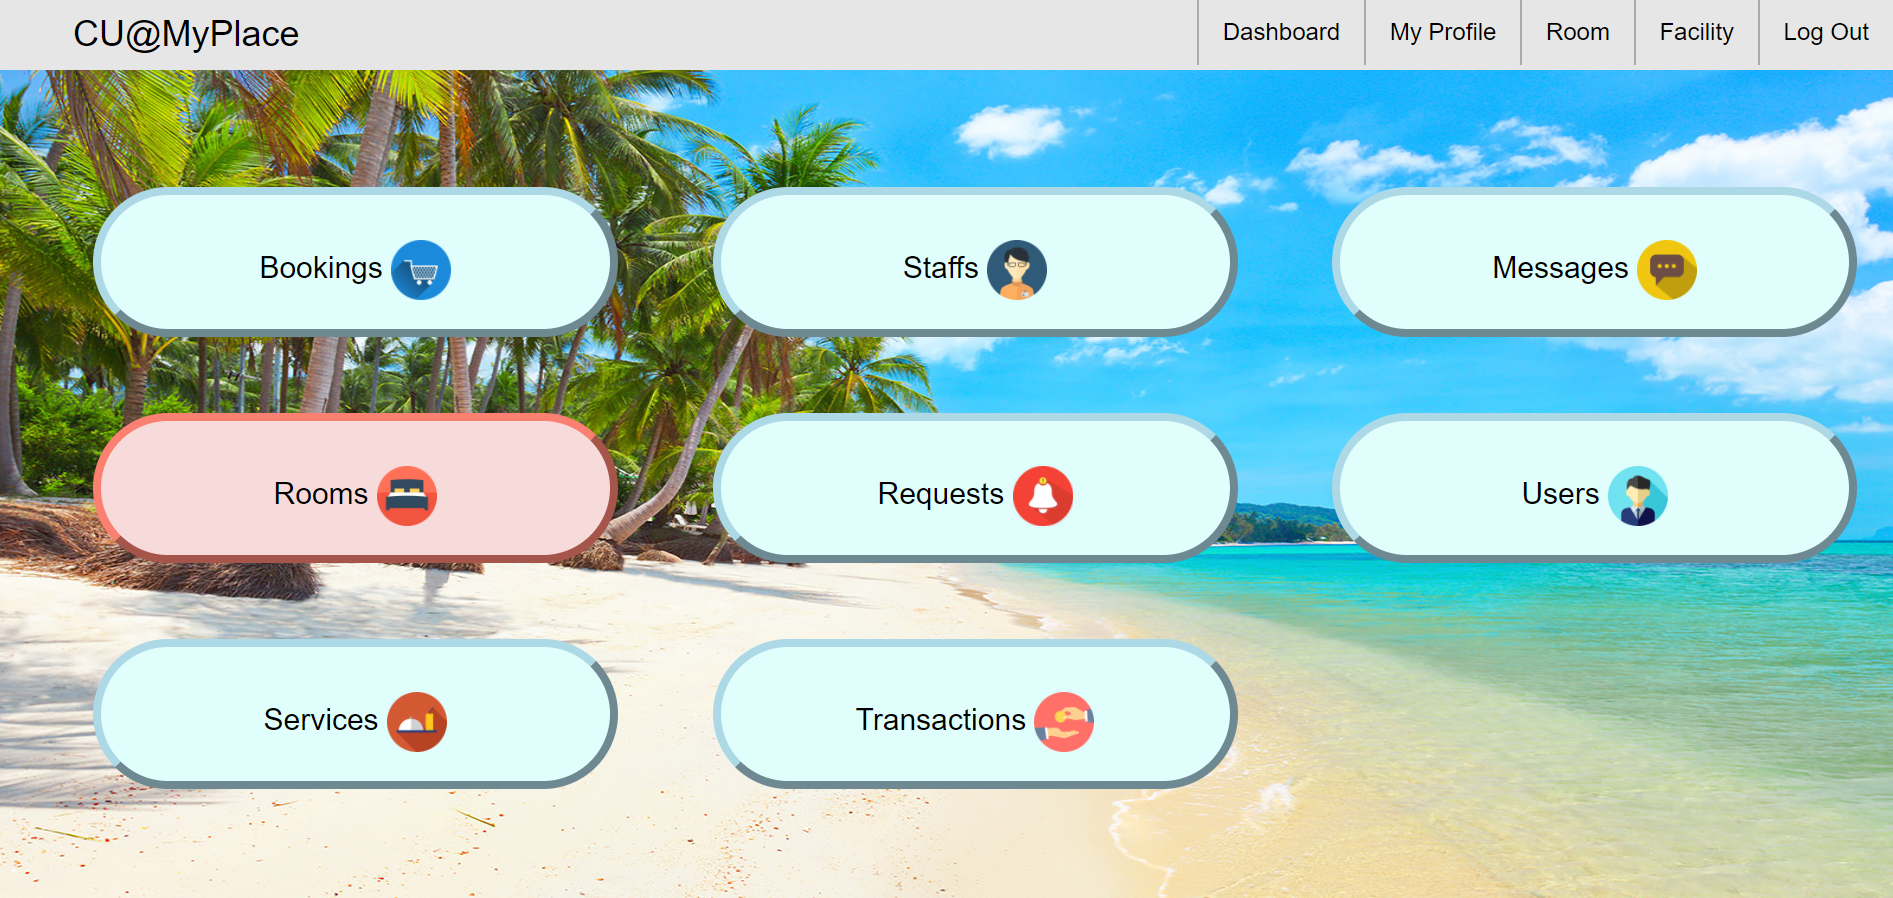
\includegraphics[width=\textwidth]{staffdashboard}
        \caption{User Interface of staffdashboard}
      \end{figure}
      \begin{figure}
        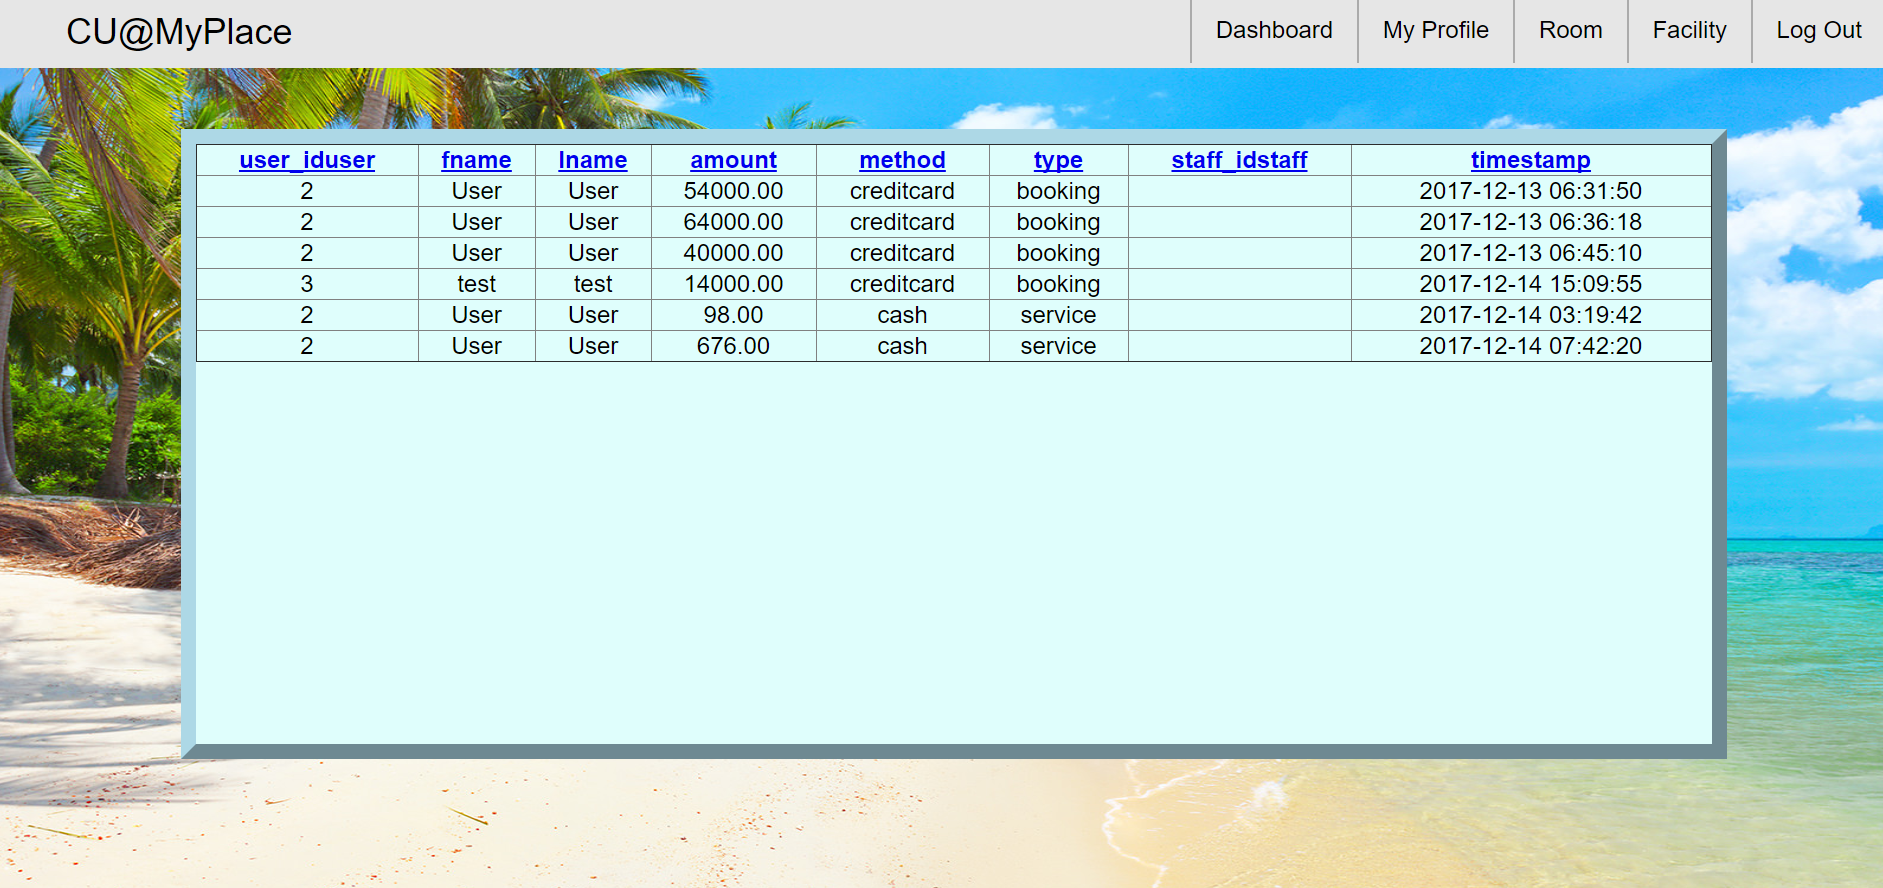
\includegraphics[width=\textwidth]{transaction}
        \caption{User Interface of transaction}
      \end{figure}
      \begin{figure}
        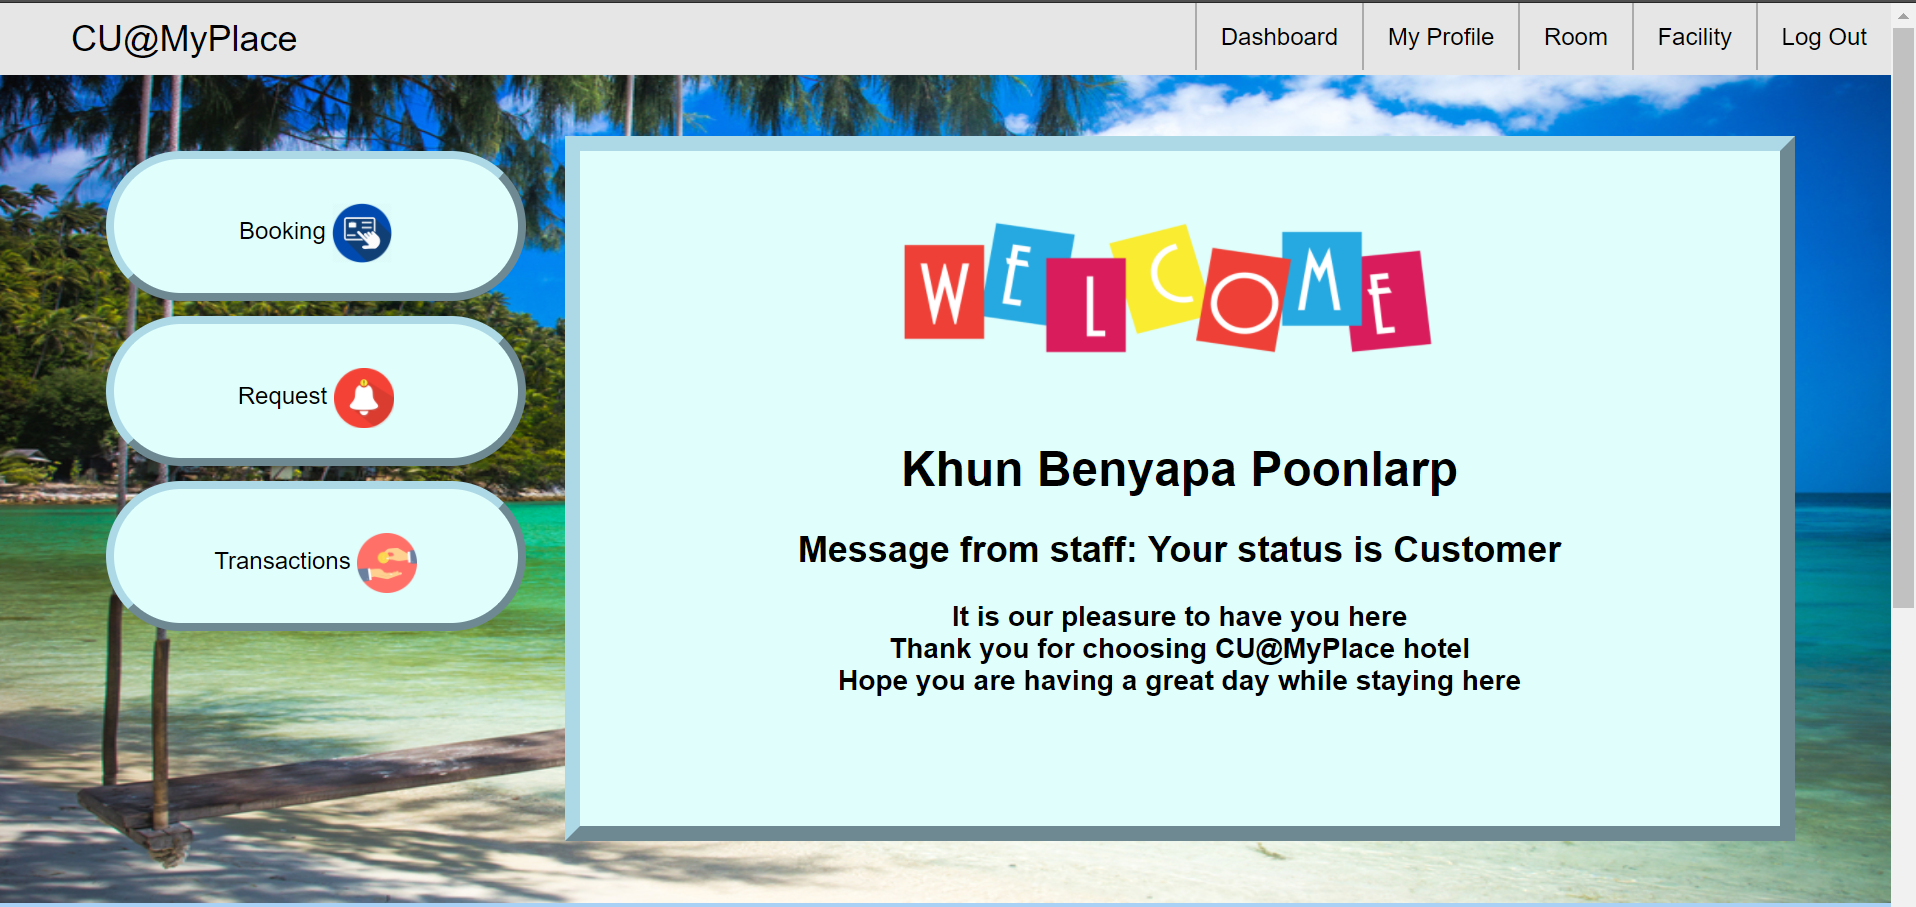
\includegraphics[width=\textwidth]{userdashboard}
        \caption{User Interface of userdashboard}
      \end{figure}

      \end{center}









\end{document}
